\subsection{Modelos relativos al servidor y usuarios}

El modelo servidor define un servidor base en el que poder recibir y gestionar los eventos generadores por nuestros dispositivos \gls{iot}. En el modelo, se crea un modelo básico \textit{JavaServer}, el cual es la mínima implementación requerida. La figura \ref{fig:modelo_iot_servidor_classes} muestra un diagrama de clases. 

\begin{figure}
	\centering
    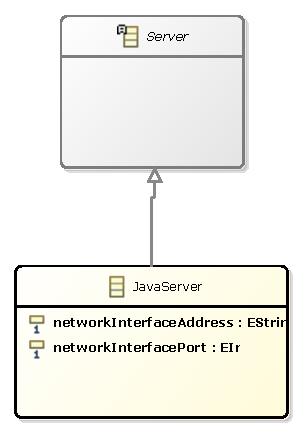
\includegraphics[height=0.3\textheight]{images/models/servers_class_diagram.pdf}
    \captionmodeloclase{Servidor}
    \label{fig:modelo_iot_servidor_classes}
\end{figure}

El modelo usuarios, cuenta con las cualidades que suelen tener los objetos tipo usuario, tales como su nombre, a que compañía pertenece, que dispositivos tiene asignados, conocer si tiene acceso a estos en un determinado momento y en que lugar están situados. La figura \ref{fig:modelo_iot_usuarios_classes} muestra un diagrama de clases.

\begin{figure}
	\centering
    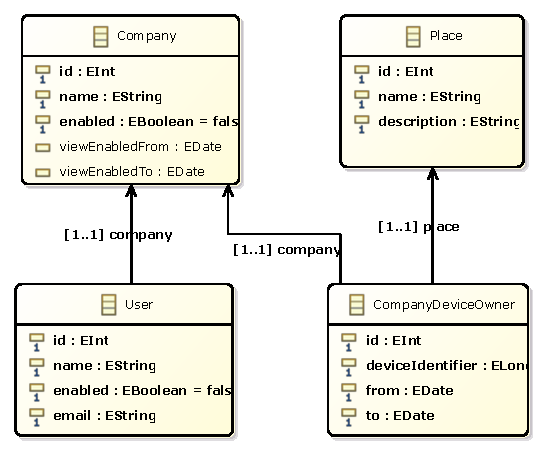
\includegraphics[height=0.3\textheight]{images/models/clients_class_diagram.pdf}
    \captionmodeloclase{Usuarios}
    \label{fig:modelo_iot_usuarios_classes}
\end{figure}
